\documentclass{article}
\usepackage[margin=1in]{geometry} 
\usepackage{amsmath}
\usepackage{graphicx}
\usepackage{caption}
\usepackage{hyperref}
\usepackage{float}
\usepackage[framed,numbered,autolinebreaks,useliterate]{mcode}
\usepackage{epstopdf}




\title{\huge ENGRD 3200 HW3} 
\author{\small Shiyao Sun, Samuel Tome \\ Group 34}


\begin{document}
\maketitle
\captionsetup{width=1 \linewidth}

\section*{Problem 1}
\subsection*{A}


\begin{figure}[H]
\centering
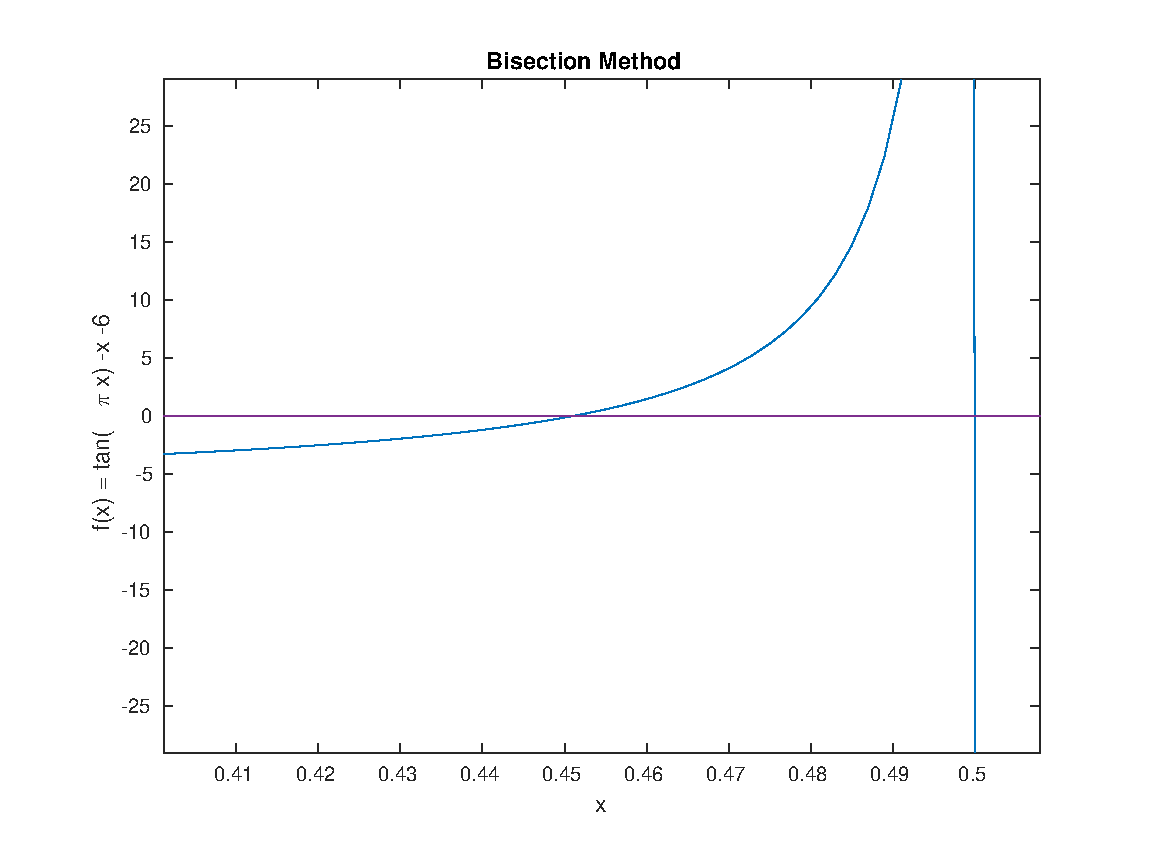
\includegraphics[width=5in]{Problem1.eps}
\caption{Detail of the first positive root of the function $f(x) = \tan(\pi x) -x -6 $.}
\end{figure}

The interval from $ [0.40,0.48]$ is a good choice for the first bracketing interval since it encloses a single sign change in the function.

The first iteration of the bisection method evaluated $f(x)$ at the lower and upper bounds of the interval and the point halfway between the two.  It looked at the sign at these three points and determined between which two it changed.  It then used these two points, which were the midpoint and the upper bound, as the lower and upper bounds for the second iteration.

\begin{table}[H]
\centering
\begin{tabular} { r  r  r r }
Iteration &  $x_l$  &  $x_u$  &  $x_r$   \\ \hline 
1 & 0.40 & 0.48 & 0.44 \\
2 & 0.44 & 0.48 & 0.46 
\end{tabular}
\end{table}

The approximate relative error for the second iteration is given by the change in $x_r$,

$$ \frac{| 0.46 - 0.44 | }{0.46} * 100\% = 4.3\% $$


The following Matlab program, modified from textbook Figure 5.7, was used to find the first root of the above function and find find number of iterations necessary to reach an acceptable tolerance.
\begin{lstlisting}
function [root,fx,ea,iter,cell]=bisect(func,xl,xu,es,maxit,varargin)
% bisect: root location zeroes
%   [root,fx,ea,iter]=bisect(func,xl,xu,es,maxit,p1,p2,...):
%      uses bisection method to find the root of func
% input:
%   func = name of function
%   xl, xu = lower and upper guesses
%   es = desired relative error (default = 0.0001%)
%   maxit = maximum allowable iterations (default = 50)
%   p1,p2,... = additional parameters used by func
% output:
%   root = real root
%   fx = function value at root
%   ea = approximate relative error (%)
%   iter = number of iterations
%   cell = table of bounds and errors

if nargin<3,error('at least 3 input arguments required'),end
test = func(xl,varargin{:})*func(xu,varargin{:});
if test>0,error('no sign change'),end
if nargin<4 || isempty(es), es=0.0001;end
if nargin<5 || isempty(maxit), maxit=50;end
iter = 0; xr = xl; ea = 100;

cell = {'Iteration','Lower bound','Upper bound','Midpoint',...
    'Approx error','f(x_r)'};

while (1)
    xrold = xr;
    xr = (xl + xu)/2;
    iter = iter + 1;
    cell{iter+1,1} = iter;
    cell{iter+1,2} = xl;
    cell{iter+1,3} = xu;
    cell{iter+1,4} = xr;
    cell{iter+1,5} = ea;
    cell{iter+1,6} = test;
    
    if xr ~= 0,ea = abs((xr - xrold)/xr) * 100;end
        test = func(xl,varargin{:})*func(xr,varargin{:});
    if test < 0
        xu = xr;
    elseif test > 0
        xl = xr;
    else
        ea = 0;
    end
    
    if ea <= es || iter >= maxit,break,end
end

root = xr; fx = func(xr, varargin{:});
\end{lstlisting}

\hspace{20pt}

\noindent which outputs:

\begin{lstlisting}
'Iteration'    'Lower bound'    'Upper bound'    'Midpoint'    'Approx error'    'f(x_r)'     
[        1]    [     0.4000]    [     0.4800]    [  0.4400]    [         100]    [   -31.2781]
[        2]    [     0.4400]    [     0.4800]    [  0.4600]    [      9.0909]    [     3.9795]
[        3]    [     0.4400]    [     0.4600]    [  0.4500]    [      4.3478]    [    -1.7438]
[        4]    [     0.4500]    [     0.4600]    [  0.4550]    [      2.2222]    [     0.1632]
[        5]    [     0.4500]    [     0.4550]    [  0.4525]    [      1.0989]    [    -0.0778]
[        6]    [     0.4500]    [     0.4525]    [  0.4512]    [      0.5525]    [    -0.0271]
[        7]    [     0.4500]    [     0.4512]    [  0.4506]    [      0.2770]    [    -0.0037]
[        8]    [     0.4506]    [     0.4512]    [  0.4509]    [      0.1387]    [     0.0076]
[        9]    [     0.4509]    [     0.4512]    [  0.4511]    [      0.0693]    [ 8.0956e-04]
[       10]    [     0.4509]    [     0.4511]    [  0.4510]    [      0.0346]    [-8.9988e-05]
[       11]    [     0.4510]    [     0.4511]    [  0.4511]    [      0.0173]    [ 6.1132e-05]
[       12]    [     0.4510]    [     0.4511]    [  0.4510]    [      0.0087]    [-4.1475e-06]
[       13]    [     0.4510]    [     0.4511]    [  0.4510]    [      0.0043]    [ 6.7542e-06]
[       14]    [     0.4510]    [     0.4511]    [  0.4510]    [      0.0022]    [ 4.9927e-07]
[       15]    [     0.4510]    [     0.4510]    [  0.4510]    [      0.0011]    [-1.0506e-07]
\end{lstlisting}

\hspace{20pt}

Because the bisection method must evaluate a function three times per iteration (once per endpoint plus the midpoint) and it took 15 iterations to reach the desired tolerance, this method had to evaluate the function a total of 45 times.


\section*{Problem 2}
\subsection*{A}

Textbook Figure 6.7 was modified to evaluate the Newton-Raphson method while also outputting information for each iteration:

\begin{lstlisting}
function [root,ea,iter,cell]=newtraph(func,dfunc,xr,es,maxit,varargin)
% newtraph: Newton-Raphson root location zeroes
% [root,ea,iter]=newtraph(func,dfunc,xr,es,maxit,p1,p2,...):
% uses Newton-Raphson method to find the root of func
% input:
% func = name of function
% dfunc = name of derivative of function
% xr = initial guess
% es = desired relative error (default = 0.0001%)
% maxit = maximum allowable iterations (default = 50)
% p1,p2,... = additional parameters used by function
% output:
% root = real root
% ea = approximate relative error (%)
% iter = number of iterations

if nargin < 3,error('at least 3 input arguments required'),end
if nargin < 4 || isempty(es),es=0.0001;end
if nargin < 5 || isempty(maxit),maxit=50;end

cell = {'Iteration','Previous estimate','New estimate','Percent approx error'};

iter = 0;

while (1)
    xrold = xr;
    cell{iter+2,2} = xr;
    xr = xr - func(xr)/dfunc(xr);
    iter = iter + 1;
    
    cell{iter+1,1} = iter;
    cell{iter+1,3} = xr;
   
    if xr ~= 0
        ea = abs((xr - xrold)/xr) * 100;
        cell{iter+1,4} = ea;
    end
    if ea <= es || iter >= maxit, break, end
end
root = xr;
\end{lstlisting}

\hspace{20pt}

\noindent which outputs the following table:

\begin{lstlisting}
'Iteration'    'Previous estimate'    'New estimate'    'Percent approx error' 
[        1]    [           0.4800]    [      0.4682]    [             2.5268]
[        2]    [           0.4682]    [      0.4570]    [             2.4363]
[        3]    [           0.4570]    [      0.4518]    [             1.1634]
[        4]    [           0.4518]    [      0.4511]    [             0.1599]
[        5]    [           0.4511]    [      0.4510]    [             0.0024]
[        6]    [           0.4510]    [      0.4510]    [         5.4277e-07]
\end{lstlisting}


\subsection*{B}

Example code from MathWorks at \href{http://www.mathworks.com/matlabcentral/fileexchange/36737-secant-method/content/secant.m}{http://www.mathworks.com/matlabcentral/fileexchange/36737-secant-method/content/secant.m} was modified to produce the secant method while also outputting information for each iteration:

\begin{lstlisting}
% It will take function and initial value as the input of function. 
% a, b are two initial guesses
% maxerr is the acceptable approximate relative error
% The function returns y and cell, where y is the root to the function
% cell is a cell array which stores the number of iteration, previous
% estimate, new estimate and relative error

function [y,cell] = secant(f,a,b,maxerr)
c = (a*f(b) - b*f(a))/(f(b) - f(a));
iter = 1;       
cell = {'iteration','Previous estimate','New estimate','relative error'};
while abs(f(c)) > maxerr
    a = b;
    b = c;
    c = (a*f(b) - b*f(a))/(f(b) - f(a));
    cell{iter+1,1} = iter;
    cell{iter+1,2} = a;
    cell{iter+1,3} = b;
    cell{iter+1,4} = abs(f(c));
    iter = iter + 1;
    if(iter == 25)
        break;
    end
end
y = c;
\end{lstlisting}

\hspace{20pt}

\noindent which gives

\begin{lstlisting}
'Iteration'    'Previous estimate'    'New estimate'    'Relative error'
[        1]    [           0.4800]    [      0.5037]    [       11.3492]
[        2]    [           0.5037]    [      0.4822]    [       14.0317]
[        3]    [           0.4822]    [      0.4845]    [        4.9946]
[        4]    [           0.4845]    [      0.4723]    [        2.7451]
[        5]    [           0.4723]    [      0.4656]    [        0.9625]
[        6]    [           0.4656]    [      0.4574]    [        0.2587]
[        7]    [           0.4574]    [      0.4529]    [        0.0322]
[        8]    [           0.4529]    [      0.4513]    [        0.0012]
[        9]    [           0.4513]    [      0.4511]    [    6.0377e-06]



\end{lstlisting}

\subsection*{C}

\subsection*{D}

The following script was used to find the first root of the equation $ f(x) = \tan(\pi x) -x -6 $ using all three methods to within an approximate relative error of $ 10^{-6} $ for the Newton-Raphson and secant methods and $ 10^{-5} $ for the bisection method.  The script then plots the approximate relative error as a function of iteration number.

\begin{lstlisting}
% Gathers together tables of iterations and relative error
% Plots these

% Create function and derivative

fx = @(x) tan(pi*x) -x -6;
df = @(x) pi*(sec(pi*x))^2 -1;

% Get bisect data
[mass blah ea iter bsect]=bisect(fx,.4,.48,.001,100);
bsect1 = cell2mat(bsect(2:16,:)); %Convert to numeric values

% Get Newton-Raphson data
[root,ea,iter,nr] = newtraph(fx,df,0.48,.0001,25);
nr1 = cell2mat(nr(2:7,:)); %Convert to numeric values

% Get secant data
[y,sc] = secant(fx,0.54,.48,.0001);
sc1 = cell2mat(sc(2:10,:)); %Convert to numeric values

close all

figure(1)
semilogy(bsect1(1:15,1),bsect1(1:15,5),'-o')
hold on
plot(nr1(1:6,1),nr1(1:6,4),'-o')
plot(sc1(1:9,1),sc1(1:9,4),'-o')
legend('Bisect','Newton-Raphson','Secant')
xlabel('Iteration')
ylabel('log_{10}Error')
hold off

\end{lstlisting}


\begin{figure}[H]
\centering
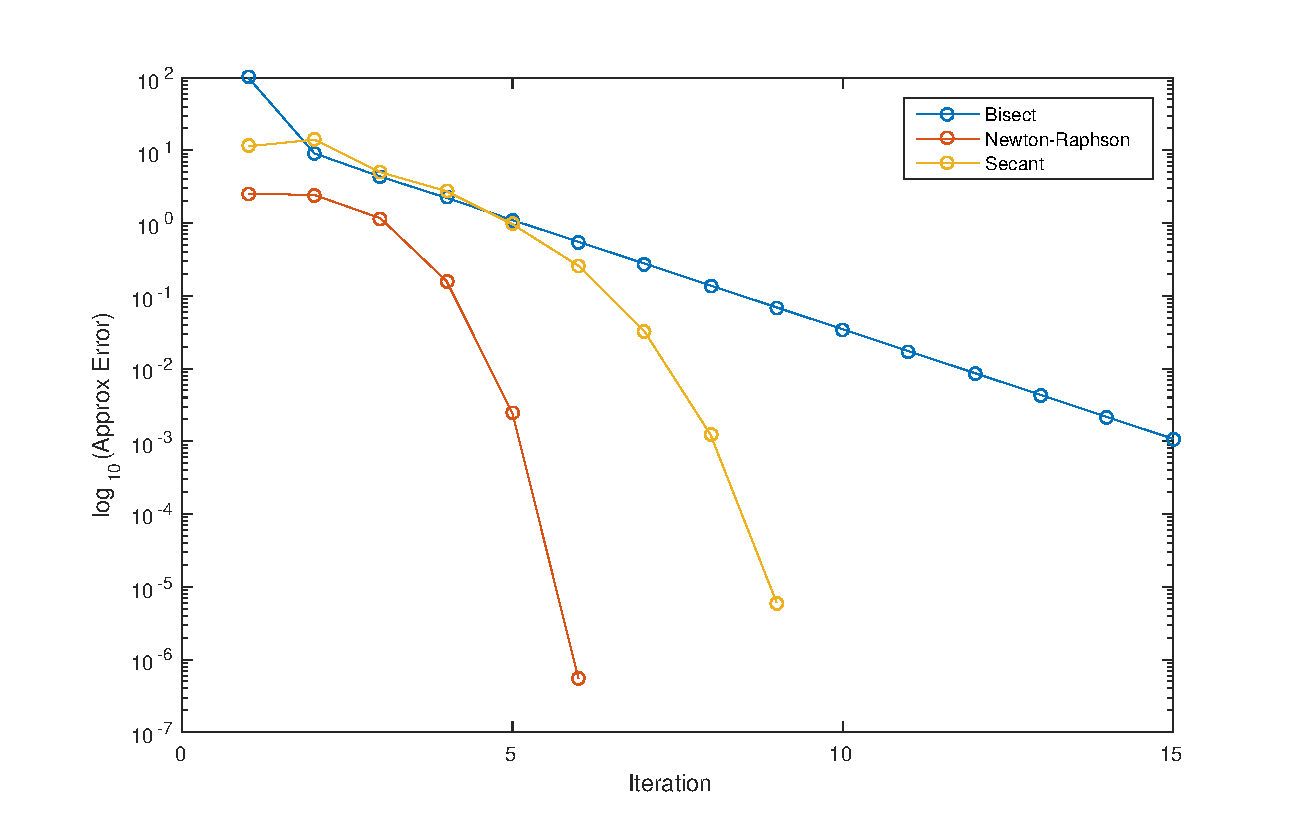
\includegraphics[width=5in]{Problem2.eps}
\caption{Approximate relative error as a function of iteration number}
\end{figure}







\end{document}